\documentclass[12pt]{article}
\usepackage[utf8]{inputenc}
\usepackage[T1]{fontenc}
\usepackage{graphicx}
\usepackage{xcolor}
\usepackage{hyperref}
\usepackage[english]{babel}
\usepackage{multicol}
%%novalidate

\usepackage{tikz}
\usepackage{calc}
\usepackage{booktabs}
%\usepackage{hyperref}

% colors
\definecolor{color1}{HTML}{000060}
%\definecolor{color1}{HTML}{8C260F}
\definecolor{color2}{HTML}{333333}


% fonts
\usepackage{fontspec}
\defaultfontfeatures{Mapping=tex-text}
\setmainfont
[BoldFont=Lato-Bold.ttf,
ItalicFont=Lato-Italic.ttf,
BoldItalicFont=Lato-BoldItalic.ttf]
{Lato-Regular.ttf}
\newfontfamily\headingfont[ItalicFont=Lato-BlackItalic.ttf]{Lato-Black.ttf}
%%%

\usepackage{geometry}
\geometry{a4paper,
hmargin=20mm,vmargin=20mm,
head=0ex,foot=3ex}

\linespread{1.3}

\usepackage[hang]{caption}
\DeclareCaptionFormat{upper}{#1#2\uppercase{#3}\par}
\captionsetup{labelfont={bf,color=color2},textfont={normalsize,color=color2},format = upper,figurename=FIGURE,tablename=TABLE}

%%% fancy sections
\usepackage{titlesec}
%\titleformat{\chapter}{\headingfont\LARGE\bfseries\scshape\color{color1}}{\thechapter}{1em}{}[\titlerule]
\titleformat{\section}{\color{color1}\headingfont\Large\bfseries\uppercase}{\thesection}{1em}{}[\titlerule]
\titleformat{\subsection}{\color{color1}\headingfont\large\bfseries\uppercase}{\thesubsection}{1em}{}
\titleformat{\subsubsection}{\color{color1}\headingfont\bfseries\uppercase}{\thesubsubsection}{1em}{}
%%%

% head and foot
\usepackage{fancyhdr}
\pagestyle{fancy}
\lhead{}
\chead{}
\makeatletter
\rhead{\color{color2}\@date}
\makeatother
\newlength{\myheight}
\lfoot{
\settoheight{\myheight}{\thepage}
\raisebox{-2ex-0.5\myheight}{
\includegraphics[height=4ex]{logo}}
}
\cfoot{\color{color2}VIET NGUYEN - Aalto University}
\rfoot{\color{color2}\thepage}
\renewcommand\headrulewidth{0pt}
\renewcommand\footrulewidth{0pt}

%%% picture on cover page
\usepackage{eso-pic}
\newcommand\BackgroundPic{%
\put(0,0){%
\parbox[b][\paperheight]{\paperwidth}{%
\vfill
\centering

\includegraphics[width=\paperwidth,height=\paperheight,%
keepaspectratio]{cover}%
\vfill
}}}
%%%
% custom titlepage
\makeatletter
\renewcommand{\maketitle}{
\thispagestyle{empty}
\AddToShipoutPicture*{\BackgroundPic}
\ClearShipoutPicture
%
\phantom{a}
\vfill
\phantom{a}\hfill
\begin{tabular}[c]{@{}p{0.7\textwidth}@{}}
      \color{white}\headingfont\LARGE\@title\\[1em]
      \color{white}\headingfont\Large\@author\\[2em]
\end{tabular}
%
\clearpage
}
\makeatother
%%%


%%% fancy boxes
\usepackage{tcolorbox}
\usepackage{wrapfig}
\def\fullboxbegin{
\bigskip
\begin{tcolorbox}[colback=color1,colframe=color1,coltext=white,arc=0mm,boxrule=0pt]
}
\def\fullboxend{\end{tcolorbox}\medskip}
%
\def\leftboxbegin{
\begin{wrapfigure}{l}{0.5\textwidth}
\begin{tcolorbox}[colback=color1,colframe=color1,coltext=white,arc=0mm,boxrule=0pt]
}
\def\leftboxend{
\end{tcolorbox}
\end{wrapfigure}
}
%
\def\rightboxbegin{
\begin{wrapfigure}{r}{0.5\textwidth}
\begin{tcolorbox}[colback=color1,colframe=color1,coltext=white,arc=0mm,boxrule=0pt]
}
\def\rightboxend{
\end{tcolorbox}
\end{wrapfigure}
}
%
\newcounter{frames}
\def\frameboxbegin#1{
\bigskip
\refstepcounter{frames}
\begin{tcolorbox}[colback=white,colframe=color1,arc=0mm,title={\MakeUppercase{\textbf{Frame \arabic{frames}}: #1}}]
}
\def\frameboxend{
\end{tcolorbox}
}
%%%

\usepackage{lipsum}
\usepackage[nottoc]{tocbibind}

%%%%%%%%%%%%%%%
% Title Page
\title{Application of Machine Learning in Self-organized Network Management}
\author{Viet Nguyen \newline Aalto University}
\date{}
%%%%%%%%%%%%%%%

\begin{document}
\maketitle

\tableofcontents
\clearpage

\section{Definition}

\subsection{Pictures used}


Self-organization as applied to cellular networks
is usually referred to Self-organizing Networks (SONs), and it
is a key driver for improving Operations, Administration, and
Maintenance (OAM) activities. (definition)
SON aims at reducing the cost of
installation and management of 4G and future 5G networks, by
simplifying operational tasks through the capability to configure,
optimize and heal itself. (benefit)
Machine Learning
(ML) has been identified as the key tool to implement autonomous
adaptability and take advantage of experience when making
decisions. (ML - SOn)

Up to 4G - hardware . 5g software 
With the advent of these software advancements,
and unprecedented levels of computational capacity, the vision
of autonomous network management can be put into practice
taking advantage of also other cross-disciplinary knowledge
advancements in the area of Machine Learning.

Network management: self-awareness, self-configuration,
self-optimization, and self-healing,

SON is a common term used to
refer to mobile network automation and minimization of human
intervention in the cellular/wireless network management.

Benefit: 1) to bring intelligence and autonomous
adaptability into cellular networks, 2) to reduce capital and
operation expenditures (CAPEX/OPEX), 3) to enhance network
performances in terms of network capacity, coverage,
offered service/experience, etc.

Problem: 1) mainly based on heuristics,
2) the automated information processing is usually limited to
low complexity solutions like triggering, 3) many operations
are still done manually (e.g. network faults are usually fixed
directly by engineers), 4) SON solutions do not really capi2
talize on the huge amount of information that is available in
mobile networks to build next generation network management
solutions, and 5) several open challenges are still unsolved,
like the problem of coordination of SON functions [15], [16],
or the proper solution of the trade-off between centralized and
distributed SON implementations

Network Functions Virtualisation (NFV) bring the economy of scale: selforganized
network management vision could be extended also
beyond the RAN segment and include all the segments
of the network, from the access to the core, while fulfilling
the requirements of different kind of vertical service instances.

Reason for machine learning:
* use of SON and of
smart network management policies is crucial and inevitable
for operators running multi-RAT, multi-vendor, multi-layer
networks, where an overwhelming number of parameters need
to be configured and optimized.
* We believe that Machine Learning (ML) can be effectively
used to allow the network to learn from experience, while improving
performance. In particular, big data analytics, through
the analysis of data already generated by the network, can
pursue the self-awareness by driving the network management
from reactive to predictive.
\section{Definition}

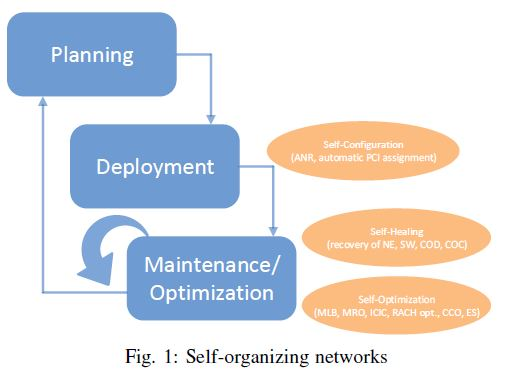
\includegraphics[]{fig1.jpg}
A Self-Organizing Network (SON) is an automation technology designed to make the planning, configuration, management, optimization and healing of mobile radio access networks simpler and faster.

Self-organizing network functionalities are commonly divided into three major sub-functional groups, each can be used in most phases of the life cycle of a cellular systems (planning, deployment,
maintenance and optimization) into: self-configuration,
self-healing and self-optimization, as depicted in Figure 1.


\subsection{Self-Configuration}
Self-configuration strives towards the "plug-and-play" paradigm in the way that new base stations shall automatically be configured and integrated into the network. This means both connectivity establishment, and download of configuration parameters are software. Self-configuration is typically supplied as part of the software delivery with each radio cell by equipment vendors. When a new base station is introduced into the network and powered on, it gets immediately recognized and registered by the network. The neighboring base stations then automatically adjust their technical parameters (such as emission power, antenna tilt, etc.) in order to provide the required coverage and capacity, and, in the same time, avoid the interference.
\subsection{Self-Optimization}
Every base station contains hundreds of configuration parameters that control various aspects of the cell site. Each of these can be altered to change network behavior, based on observations of both the base station itself and measurements at the mobile station or handset. One of the first SON features establishes neighbor relations automatically (ANR) while others optimize random access parameters or mobility robustness in terms of handover oscillations. A very illustrative use case is the automatic switch-off of a percent of base stations during the night hours. The neighboring base station would then re-configure their parameters in order to keep the entire area covered by the signal. In case of a sudden growth in connectivity demand for any reason, the "sleeping" base stations "wake up" almost instantaneously. This mechanism leads to significant energy savings for operators.
\subsection{Self-healing}
When some nodes in the network become inoperative, self-healing mechanisms aim at reducing the impacts from the failure, for example by adjusting parameters and algorithms in adjacent cells so that other nodes can support the users that were supported by the failing node. In legacy networks, the failing base stations are at times hard to identify and a significant amount of time and resources is required to fix it. This function of SON permits to spot such a failing base stations immediately in order to take further measures, and ensure no or insignificant degradation of service for the users.


\section{ML}
Class of problem can be addressed with ML when managing the network autonomously are:
\begin{itemize}
	\item Variable estimation or classification: The tasks belonging
	to this class of problem aim at e.g. estimating the QoS
	or the QoE of the network, at predicting performances or
	behaviours of the network, by learning from the analysis
	of data obtained from past behaviours of the network. NM
	and SON functions where these tasks are useful are QoS
	8
	estimation and other MDT use cases, the prediction of
	behaviours to optimize network parameters, etc. Solutions
	to these problems can be translated into finding the
	relationship between one variable and some others, or
	Identifying which class of a set of pre-defined classes
	the data belongs to. Solutions are then to be found in
	the SL literature, with both regression and classification
	tasks.
	\item Diagnosis of network faults or misbehaviours: The tasks
	belonging to this class of problems aim at detecting issues
	ongoing in the network, which may be associated to faults
	and anomalous setting of network parameters. This kind
	of problems relates to self-healing issues and solutions
	can be found in UL literature, and in particular in the
	anomaly detection solution.
	\item Dimensionality reduction: The network generates continuously
	a huge amount of data. For an appropriate processing
	and to extract useful information, it is convenient to
	eliminate the noise present in the data base, by reducing
	the dimensionality of data. Solutions to this problem are
	to be found in the UL literature, and specifically among
	the dimensionality reduction solutions.
	\item Pattern identification, grouping: The tasks belonging to
	this class aim at identifying patterns, group of nodes
	with similar characteristics, according to some kind of
	criteria. An objective may be to apply to them similar
	optimization approaches. Self-configuration use cases are
	intuitive application for these issues. Solutions to these
	problems can be translated into learning the set of classes
	the data belongs to. UL literature offers solutions in the
	area of clustering.
	\item  Sequential decision problems for online parameter ad-
	justment: This class of problems is extremely common
	in the area of autonomous management, where we face
	control decision problems to online adjust network parameters,
	with the objective to meet certain performance
	targets. This kind of decision problems, where we learn
	the most appropriate decision online, based on the reaction
	of the environment to the actions the network is
	taking, can be addressed through RL solutions. All selfoptimization
	use cases can be addressed through these
	solutions, as well as COC problems.
\end{itemize}
\section{Address SON and NM through ML}
a huge amount of data from normal
operations of mobile network can be exploited to find patterns and extract useful
information:


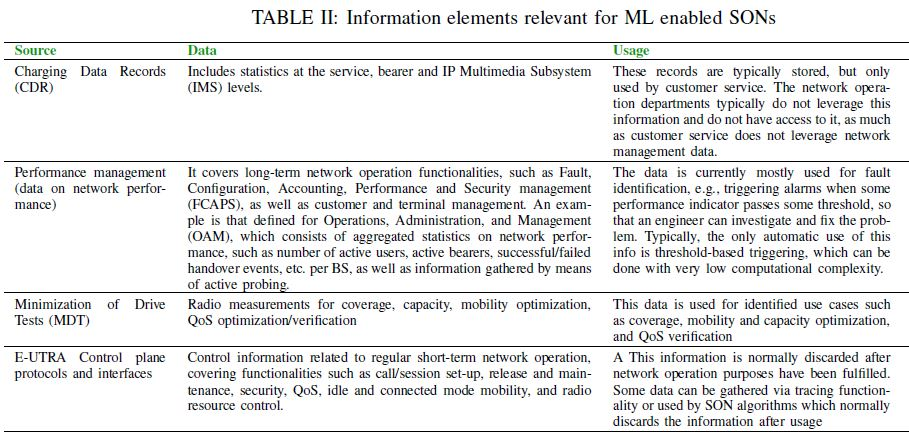
\includegraphics[width=1\textwidth]{table2.jpg}

\noindent Table IV
summarizes the main use cases of ML in each SON and Network management function and classifies them
per 3GPP use case, technique and specific algorithm

\begin{itemize}
	\item Mobility Load Balancing:The majority of applications fall in the area of Reinforcement learning (RL), as the main problem to solve is a sequential decision problem
	about how to set configuration parameters, which optimize
	network performance and user experience. 
	An example of a
	RL application for MLB use case can be found in [135].
	Here the authors present a distributed Q-learning approach
	that learns for each load state the best MLB action to take,
	while also minimizing the degradation in HO metrics. Another
	option to take advantage also of fuzzy logic capabilities of
	dealing with heterogeneous sources of information is provided
	in [136], where fuzzy logic is combined with Q-learning in
	order to target the load balancing problem. For similar reasons,
	fuzzy logic is also proposed in [137] to enhance the network
	performance by tuning HO parameters at the adjacent cells.
	Approaches incorporating fuzzy logic with RL capabilities
	have the advantage to capture the uncertainty existing in real
	world complex scenarios, while schemes considering only
	learning approaches may be limited by the fixed variable
	definition. When combining fuzzy logic with RL, also the
	subjectivity with which the fuzzy variable may be defined
	is overcome by the adjusting capabilities of the learning.
	Alternatively, a centralized solution is approached in [138],
	where a central server in the cellular network determines all
	HO margins among cells by means of a dynamic programming
	approach. Besides RL, also clustering schemes have been
	proposed in this area, to group cells with similar characteristics
	and provide for them similar configuration parameters [139].
	Considering clustering in large realistic scenarios is an added
	value to reduce computational complexity and take advantage
	of what is learnt in other regions of the network where we
	observe similar environment characteristics.
	\item Mobility Robustness Optimization: Also for the case of
	MRO, we find in literature different solutions based on RL to
	solve a control decision problem. In [141], [142], the authors
	focus on the optimization of the users’ experience and of
	the HO performance. In [141] the authors take advantage of
	the Q-learning approach to effectively reduce the call drop
	rates, whereas in [142], unlike other solutions that assume a
	general constant mobility, the authors adjust the HO settings in
	response to the mobility changes in the network by means of
	a distributive cooperative Q-learning. Differently from [141],
	[142], in [143], the authors take advantage also of fuzzy logic
	capabilities. These solutions are based on control optimization
	of HO parameters through RL, so they propose similar
	solutions to those found in the literature of MLB. In this
	case we can do the same considerations about the advantages
	of considering fuzzy logic in order to gain in flexibility in
	the uncertain and complex real network context. Different
	approaches in turn, address the problem by identifying successful
	HO events, through solutions based on unsupervised
	learning. In particular, the works of [144] and [145] propose an
	approach to HO management based on UL and SOM analysis.
	The idea is to exploit the experience gained from the analysis 
	of data of the network based on the angle of arrival and the
	received signal strength of the user, to learn specific locations
	where HOs have occurred and decide whether to allow or
	forbid certain handovers to enhance the network performance.
	The solutions enable self-tuning of HO parameters to learn
	optimal parameters’ adaptation policies. Similarly, in [146] the
	authors exploit the huge amount of information generated in
	the network to predict user traffic distribution. In particular,
	they take advantage of semi-Markov model for spatiotemporal
	mobility prediction in cellular networks. Finally, the works in
	[147]–[150], propose schemes to make predictions about UE’s
	mobility, which allows to anticipate smart HO decisions.
	\item Coverage and Capacity Optimization: In case of CCO,
	different approaches in literature focus on RL solutions based
	on continuous interactions with the environment, oriented to
	online adjusting antenna tilts and transmission power levels
	through TD learning approaches. In [151] and [152] a fuzzy Qlearning
	approach to optimize the complex wireless network,
	by learning the optimal antenna tilt control policy has been
	proposed, and a similar approach is followed also in [153]
	and [154]. In addition, they also propose to combine fuzzy
	logic with Q-learning, in order to deal with continuous input
	15
	and output variables. [153] also proposes a central control
	mechanism, which is responsible to initiate and terminate the
	learning optimization process of every learning agent deployed
	in each eNB. Finally, [154] innovates with respect to other
	approaches since in order to adjust the antenna tilt and transmission
	power parameters, it considers the load distribution
	of the different cells involved in the optimization process, and
	introduces novel mechanisms to facilitate cooperative learning
	among the different SON entities.
	\item Inter-cell Interference Coordination: Similarly to the
	CCO case, ML has been proposed in the literature of ICIC use
	case as a valid solution, where RL is the principle used tool,
	with special emphasis to TD methods, in order to target the
	optimization of control parameters. Several works target the
	problem to minimize the interference among cells by using the
	most common TD learning method, Q-learning [155]–[158].
	The work in [155] is related to control inter-cell interference in
	a heterogeneous femto-macro network. The work combines information
	handled by the multi-user scheduling with decisions
	taken by a learning agent based on Q-learning, which tries to
	control the cross-tier interference per resource block. [156]
	proposes a distributed solution for ICIC in OFDMA networks
	based on a Fuzzy Q-learning implementation. The proposed
	solution achieves joint improvement for all users, i.e., the
	improvements of users with bad quality does not come at the
	expense of users with good quality. Moreover, a decentralised
	Q-learning framework for interference management in small
	cells is proposed in [157]. The authors focus on a use case in
	which the small cell networks aim to mitigate the interference
	caused to the macro-cell network, while maximizing their own
	spectral efficiencies. Finally, in [158] also a decentralized Qlearning
	approach for interference management is presented.
	The goal is to improve the systems performance of a macrocellular
	network overlaid by femto-cells. In order to improve
	the time of convergence, a mitigation approach has been
	introduced, allowing them to have significant gains in terms
	of throughput for both, macro and femto users. Interesting
	trade-offs can be studied to compare centralized vs. distributed
	solutions. In the novel context of small cells distributed solutions
	to interference management are to be preferred over more
	complex centralized solutions, but convergence and instability
	approaches may appear to affect the TD learning schemes,
	compromising system performances [155].
	\item Energy Savings: Energy savings schemes for wireless
	cellular systems have been proposed in the past, enabling cells
	to go into a sleep mode, in which they consume a reduced
	amount of energy. In order to reduce the energy consumption
	of the eNBs, we can found several works related to ML
	techniques. An example of that can be found in [159], where
	the authors take advantage of RL to propose a decentralized Qlearning
	approach to allow energy savings by learning a policy
	by the iterations with the environment taking into account
	different aspects over time, such as the daily solar irradiation.
	Also, in [160], the authors switch off some underutilized cells
	during off peak hours. The proposed approach optimizes the
	number of base stations in dense LTE pico cell deployments
	in order to maximize the energy saving. For the purpose,
	they use a combination of Fuzzy Logic, Grey Relational
	Analysis and Analytic Hierarchy Process tools to trigger the
	switch off actions, and jointly consider multiple decision
	inputs for each cell. This last work uses smart decision theory
	approaches, which though are not able to take advantage of
	the previous decisions made in the same environment, as in
	turn does the work proposed in [159], as a result of the TD
	learning approach. This allows that the work in [159] offers
	a more solid solution, considering also past information in
	the decision. Also for HetNets, we find several works, such
	as, [161], [162], where the authors take advantage of KPIss
	available in the network for the construction of different kind
	of databases to analyse the potential gains that can be achieved
	in clustered small cell deployments.
	\item Cell Outage Compensation: The literature already offers
	different works targeting the problem of COC. For this use
	case RL has been proven as a valid solution since it is a
	continuous decision making/control problem. In this context
	a contribution in the area of self-healing has been presented
	in [163], [164], where the authors present a complete solution
	for the automatic mitigation of the degradation effect of the
	outage by appropriately adjusting suitable radio parameters
	of the surrounding cells. The solution consists of optimizing
	the coverage and capacity of the identified outage zone, by
	adjusting the gain of the antenna due to the electrical tilt
	and the downlink transmission power of the surrounding
	eNBs. To implement this approach, the authors propose a RL
	based on actor-critic theory to take advantage of its capability
	of making online decisions at each eNB, and of providing
	decisions adapting to the evolution of the scenario in terms
	of mobility of users, shadowing, etc., and of the decisions
	made by the surrounding nodes to solve the same problem.
	A COC contribution also based on ML is targeted in [165],
	where fuzzy logic is proposed as the driving techniques to
	fill a coverage gap. The authors show performance gains by
	using different parameters, such as, the power transmission,
	the antenna tilt, and a combination of the two schemes. These
	two works are compared in [163] and the work in [163] is
	proven superior thanks to the ability to learn from the past
	experience introduced by the RL actor-critic approach.
	\item Cell Outage Detection: As we already mentioned, COD
	aims to autonomously detect cells that are not operating
	properly due to possible failures. For this kind of problem,
	anomaly detection algorithms offer an interesting solution
	that allows to identify outliers measurements, which can be
	highlighting a hidden problem in the network. Proposals of
	solutions for this problem can be found in [166] and [167]. In
	particular, [166] presents a solution based on diffusion maps,
	by means of clustering schemes, capable of detecting anomalous
	behaviours generated by a sleeping cell. [167] presents
	a solution based on fuzzy logic for the automatic diagnosis
	of a troubleshooting system. In order to determine if there is
	a failure, the authors propose a controller, which receives as
	an inputs a set of representative KPIs. A similar approach is
	presented by [168], where the authors present an automated
	diagnosis model for Universal Mobile Telecommunications
	System (UMTS) networks based on Naive Bayesian classifier,
	and where the model uses both network simulator and real
	UMTS network measurements. In the context of this king of
	16
	classifiers , the works in [174], [175], also take advantage of
	NB for automated diagnosis based on different inputs network
	performances. The work in [169] addresses both the case
	of outage and the one where in turn the cell can provide
	a certain level of service, which though does not allow to
	fulfil the expected UEs requirements. The approach relies on
	ensemble methods to train KPIs extracted by human operators
	to make informed decisions. In [185], the authors consider
	large data sets to identify anomaly behaving base station. They
	proposed an algorithm consisting of preprocessing, detection
	and analysis phases. The results show that by using dimensionality
	reduction and anomaly detection techniques irregularly
	behaving base stations can be detected in a self-organized
	manner. In [164] data gathered through MDT reports is used
	for anomaly detection purposes. Furthermore, the works of
	[171]–[173] take advantage of k-NN algorithm to propose a
	self-healing solution, in particular to tackle the fault detection
	domain. Finally, in [170], the authors consider a HetNet and
	they take advantage of HMM to automatically capture the
	dynamic’s of four different states and probabilistically estimate
	if there exist a possible failure.
	\item SON Conflicts Coordination: As the deployment of
	stand-alone SON functions is increasing, the number of conflicts
	and dependencies between them also increases. Hence,
	an entity has been proposed for the coordination of this kind
	of conflicts. In this context, current literature includes several
	works based on ML. In [176] the authors focus on the classification
	of potential SON conflicts and on discussing the valid
	tools and procedures to implement a solid self-coordination
	framework. Q-learning, as a RL method, has been proposed
	in [177] to take advantage of experience gained in past
	decisions, in order to reduce the uncertainty associated with
	the impact of the SON coordinator decisions when picking an
	action over another to resolve conflicts. In [178], the authors
	use Q-learning to deal with the conflict resolution between
	two SON instances. Decision trees have been proposed in
	[186] to properly adjust Remote Electrical Tilt (RET) and
	transmission power. Additionally, in [179] the authors provide
	a functional architecture that can be used to deal with the
	conflicts generated by the concurrent execution of multiple
	SON functions. They show that the proposed approach is
	general enough to model all the SON functions and their
	derived conflicts. First they introduce these SON functions
	in the context of the general SON architecture, together with
	high-level examples of how they may interfere. Second, they
	define the state and action spaces of the global MDP that
	models the self-optimization procedure of the overall RAN
	segment. Finally, they show that the global self-optimization
	problem can be decomposed onto as many Markov decision
	sub-processs (subMDPs) as SON functions.
	\item Minimization of Drive Tests: The great majority of
	literature using the MDT functionality to target MDT use
	cases, takes advantage of supervised and unsupervised learning
	techniques to provide different solutions for the different use
	cases. An example of that can be observed in [180], [181],
	where the authors address the QoS estimation by selecting
	different KPIs and correlating them with common nodes
	measurements, to establish whether a UE is satisfied with
	the received QoS. A similar objective is targeted in [110],
	however, differently from the previous works, here the authors
	focus on multi layer heterogeneous networks, so in a more
	complex and realistic scenario than the traditional macrocell
	one. In particular, they present an approach, based on regression
	models, which allows to predict QoS in heterogeneous
	networks for UEs, independently of the physical location of
	the UE. This work is extended in [182] by taking into account
	the most promising regression models, but also analysing
	dimensional reduction techniques. By doing PCA/SPCA on the
	input features, and promoting solutions in which only a small
	number of input features capture most of the variance, the
	number of random variables under consideration is reduced.
	Based on previous results, in [111], [183] the same authors
	define a methodology to build a tool for smart and efficient
	network planning, based on QoS prediction derived by proper
	data analysis of UE measurements in the network.
	Moreover, the work in [187] presents a system based on
	a fuzzy logic controller to improve network performances by
	adjusting antenna tilts values in a LTE system. Differently
	from previous works, the authors consider the use of call
	traces to identify the level of coverage, overshooting and
	overlapping problems, which are the inputs to the algorithm.
	Also, in [188], the same authors take advantage of connection
	traces (signal strength, traffic, and resource utilization measurements)
	to improve the network infrastructure in terms of
	spectral efficiency. The proposed method is designed to be
	integrated in commercial network planning tool. Finally, in
	[189] the authors take advantage of the MDT measurements
	to build a Radio Environment Map (REM) by applying spatial
	interpolation techniques (Bayesian kriging). The REM (Radio
	Environmental Map) is then used to detect coverage holes and
	predict the shape of those areas.
	\item Core Networks: As we already mentioned in section
	II, the operational aspects of core networks elements can be
	enhanced through, for example, the automatic configuration of
	the neighbour cell relations function. In this regard, the idea of
	applying ML to this function is not new. In [184] the authors
	study the benefits of using ML to root-cause analysis of session
	drops, as well as drop prediction for individual sessions. They
	present an offline Adaboost and SVM method to create a
	predictor, which is in charge of eliminating/mitigating the
	session drops by using real LTE data.
	\item Virtualized and Software Define Networks: Also when
	we go beyond the RAN and we focus on the network in
	general, ML concepts have already been proposed in different
	works to build cognitive based techniques to operate the
	network. An example of these proposals is well summarized
	by [190]. In this work, a Knowledge Plane is advocated, which
	would bring many advantages to the networks in terms how the
	network is operated, automated, optimized and troubleshooted.
	Conceptually this vision is aligned with different others proposals
	in other areas, such as the black-box optimization [191],
	the autonomic self-x architectures [192], or the work presented
	in [193]. In this context, the work in [194] analyzes the reasons
	why the vision proposed in [190] has still not been brought to
	reality, and the main reason that they find is in the challenges
	that appear when it comes to autonomously manage a network
	17
	in a distributed fashion. In particular, the work argues that
	the emerging trend of centralization in control brought by the
	novel SDN vision, will significantly reduce this complexity
	and favour the realization of the ML vision in the network.
	As a result, in [194] some initial experimental results based
	on the vision defined in [190] are brought into reality in the
	context of a SDN based architecture. Further work in this
	area is carried put in the context of different European H2020
	projects [6]. The work in [195] presents a novel cognitive
	management architecture that manages multiple use cases,
	like the Service Level Agreement (SLA) and the Mobility
	Quality Predictor. Both use cases are tackled using machine
	learning approaches, the Long Short Term Memory, and a per
	user bandwidth predictor. The work in [196] implements SLA
	through ML approaches. It uses an ANN for evaluation of
	cognitive SLA enforcement of networking services involving
	Virtualized Network Functions and SDN controllers.
	
\end{itemize}

\section{Reference}
\begin{multicols}{2}
\noindent [134] M. Peng, D. Liang, Y. Wei, J. Li, and H. H. Chen, “Self-configuration
and self-optimization in LTE-advanced heterogeneous networks,” IEEE
Communications Magazine, vol. 51, no. 5, pp. 36–45, 2013. \\ \noindent 
[135] S. S. Mwanje, A. Mitschele-Thiel, “Minimizing Handover Performance
Degradation Due to LTE Self Organized Mobility Load Balancing,”
77th IEEE Conference on Transactions on Vehicular Technology (VTC
Spring), pp. 1–5, 2013. \\ \noindent 
[136] P. Mu˜noz, R. Barco, I. de la Bandera, “Optimization of load balancing
using fuzzy Q-Learning for next generation wireless networks,” Expert
Systems with Applications, Elsevier, vol. 40, pp. 984–994, 2013.\\ \noindent 
[137] P. Mu˜noz, R. Barto, I. de la Bandera, “Load Balancing and Handover
joint optimization in LTE networks using Fuzzy logic Reinforcement
Learning,” Computer Networks Elsevier, 2014.\\ \noindent 
[138] J. Suga, Y. Kojima, M. Okuda, “Centralized Mobility Load Balancing
Scheme in LTE Systems,” 8th International Symposium on Wireless
Communication Systems, Aachen, 2011.\\ \noindent 
\\ \noindent [139] E. Bergner, “Unsupervised Learning of Traffic Patterns in Self-
Optimizing 4th Generation Mobile Networks,” Master of Science The-
sis, KTH Computer Science and Communications, Stockholm, Sweden,
2012.
\\ \noindent [140] C. A. S. Franco, J. R. B. de Marca, “Load balancing in self-organized
heterogeneous LTE networks: A statistical learning approach,” IEEE
Latin-American Conference on Communications (LATINCOM), pp. 1–
5, 2015.
\\ \noindent [141] W. Qin, Y. Teng, M. Song, Y. Zhang, and X. Wang, “A Q-learning approach
for mobility robustness optimization in LTE-SON,” 15th IEEE
International Conference on, Communication Technology (ICCT), pp.
818–822, 2013.
\\ \noindent [142] S. S. Mwanje, A. Mitschele-Thiel, “Distributed cooperative Q-learning
for mobility-sensitive handover optimization in LTE SON,” IEEE
Symposium the Computers and Communication (ISCC), pp. 1–6, 2014.
\\ \noindent [143] P. Mu˜noz, R. Barco, and I. de la Bandera, “On the Potential of Handover
Parameter Optimization for Self-Organizing Networks,” IEEE
Transactions on Vehicular Technology, 2013.
\\ \noindent [144] N. Sinclair, D. Harle, I. A. Glover, J. Irvine, R. C. Atkinson, “Parameter
Optimization for LTE Handover using an Advanced SOM Algorithm,”
IEEE Conference on Transactions on Vehicular Technology (VTC),
2013.
\\ \noindent [145] N. Sinclair, D. Harle, I. Glover, J. Irvine, and R. Atkinson, “An
advanced SOM algorithm applied to handover management within
LTE,” IEEE Transactions on Vehicular Technology, pp. 183–1894,
2013.
\\ \noindent [146] H. Farooq, A. Imran, “Spatio-temporal Mobility Prediction in Proactive
Self-Organizing Cellular Networks,” IEEE Communications Letters,
vol. 21, no. 2, pp. 370–373, 2017.
\\ \noindent [147] Z. Ali, N. Baldo, J. Mangues-Bafalluy, and L. Giupponi, “Machine
learning based handover management for improved qoe in LTE,”
IEEE/IFIP Network Operations and Management Symposium, pp. 794–
798, 2016.
\\ \noindent [148] E. Ostlin, H. J. Zepernick, H. Suzuki, “Macrocell radio wave propagation
prediction using an artificial neural network,” IEEE Vehicular
Technology Conference (VTC Fall), p. 57, 2004.
\\ \noindent [149] A. Quintero and O. Garc´ıa, “A profile-based strategy for managing user
mobility in third-generation mobile systems,” IEEE Communications
Magazine, pp. 134–139, 2004.
\\ \noindent [150] K. Majumdar and N. Das, “Mobile user tracking using a hybrid neural
network,” in Wireless Networks, pp. 275–284, 2005.
\\ \noindent [151] R. Razavi, S. Klein, H. Claussen, “A fuzzy reinforcement learning
approach for self-optimization of coverage in LTE networks,” Bell Labs
Tachnical Journal, vol. 15, pp. 153–175, 2010.
\\ \noindent [152] M. Naseer ul Islam, A. Mitschele-Thiel, “A Cooperative Fuzzy Qlearning
for Self-Organized Coverage and Capacity Optimization,”
IEEE 23rd International Symposium on Personal Indoor and Mobile
Radio Communications (PIMRC), Sept 2012.
\\ \noindent [153] J. Li, J. Zeng, X. Su, W. Luo, J. Wang, “Self-Optimization of Coverage
and Capacity in LTE Networks Based on Central Control and
Decentralized Fuzzy Q-Learning,” International Journal of Distributed
Sensor Networks, Hindawi, 2012.
\\ \noindent [154] S. Fan, H. Tian, and C. Sengul, “Self-optimization of coverage and
capacity based on a fuzzy neural network with cooperative reinforcement
learning,” Journal on Wireless Communications and Networking,
2014.
\\ \noindent [155] A. Galindo-Serrano, L. Giupponi, G. Auer, “Distributed Learning
in Multiuser OFDMA Femtocell Networks,” 73rd IEEE Vehicular
Technology Conference (VTC Spring), pp. 1–6, 2011.
\\ \noindent [156] M. Dirani and Z. Altman, “A cooperative reinforcement learning
approach for inter-cell interference coordination in OFDMA cellular
networks,” 8th Int Modeling and Optimization in Mobile, Ad Hoc and
Wireless Networks (WiOpt), pp. 170–176, 2010.
\\ \noindent [157] M. Bennis, S. M. Perlaza, P. Blasco, “Self-Organization in Small Cell
Networks: A Reinforcement Learning Approach,” IEEE Transactions
on Wireless Communications, vol. 12, no. 7, 2013.
\\ \noindent [158] M. Simsek, A. Czylwik, A. Galindo-Serrano, L. Giupponi, “Improved
decentralized Q-learning algorithm for interference reduction in LTEfemtocells,”
5th International Workshop on Self-Organizing Networks
IWSON, Glasgow, 2015.
\\ \noindent [159] M. Miozzo, L. Giupponi, M. Rossi, P. Dini, “Distributed Q-Learning
for Energy Harvesting Heterogeneous Networks,” IEEE ICC 2015
Workshop on Green Communications and Networks with Energy Har-
vesting, Smart Grids, and Renewable Energies, June 2015.
\\ \noindent [160] A. Dudnikova, P. Dini, L. Giupponi, D. Panno, “Multiple Criteria plus
Fuzzy Logic Switch Off Method for Dense Heterogeneous Networks,”
20th IEEE International Workshop on Computer Aided Modelling and
Design of Communication Links and Networks, Guildford (UK), 2015.
\\ \noindent [161] E. Ternon, P. Agyapong, L. Hu, A. Dekorsy, “Energy Savings in Heterogeneous
Networks with Clustered Small Cell Deployments,” 11th
IEEE International Symposium on Wireless Communications Systems
(ISWCS), 2014.
\\ \noindent [162] E. Ternon, P. Agyapong, L. Hu, and A. Dekorsy, “Database-aided
Energy Savings in Next Generation Dual Connectivity Heterogeneous
Networks,” IEEE WCNC’14 Track 3: Mobile and Wireless Networks,
2014.
\\ \noindent [163] J. Moysen and L. Giupponi, “A Reinforcement Learning based solution
for Self-Healing in LTE networks,” 80th IEEE Vehicular Technology
Conference (VTC Fall), Vancouver, Canada, 2014.
\\ \noindent [164] O. Onireti, A. Zoha, J. Moysen, A. Imran, L. Giupponi, M. Ali
Imran, A. Abu-Dayya, “A Cell Outage Management Framework for
Dense Heterogeneous Networks,” IEEE Transactions on Vehicular
Technology, vol. 64, pp. 2097–2113, April 2015.
\\ \noindent [165] A. Saeed, O. G. Aliu, M. A. Imran, “Controlling Self Healing Cellular
Networks using Fuzzy Logic,” IEE Wireless Communications and
Networking Conference (WCNC), Paris, France, April 2012.
\\ \noindent [166] F. Chernogorov, J. Turkka, T. Ristaniemi, A. Averbuch, “Detection of
Sleeping Cells in LTE Networks Using Diffusion Maps,” IEEE 73rd
Vehicular Technology Conference (VTC Spring), pp. 1–5, may 2011.
\\ \noindent [167] E. J. Khatib, R. Barco, A. Gomez-Andrades, I. Serrano, “Diagnosis
based on genetic fuzzy algorithms for LTE Self-Healing,” IEEE Trans-
actions on Vehicular Technology, 2015.
\\ \noindent [168] R. M. Khanafer, B. Solana, J. Triola, R. Barco, L. Moltsen, Z. Altman,
P. Lazaro, “Automated Diagnosis for UMTS Networks Using Bayesian
Network Approach,” IEEE Transactions on Vehicular Technology,
vol. 57, 2008.
\\ \noindent [169] G. F. Ciocarlie, S. N. Sanneckaczki, “Detecting Anomalies in Cellular
Networks Using an Ensemble Method,” 9th CNSM and Workshops,
2013.
\\ \noindent [170] A. Multazamah, S. Navrati, R. Abhishek, “Efficient Cell Outage
Detection in 5G Het-Nets Using Hidden Markov Model,” IEEE Com-
munications Letters, vol. 20, no. 3, 2016.
\\ \noindent [171] W. Xue, M. Peng, Y. Ma, and H. Zhang, “Classification-based approach
for cell outage detection in self-healing heterogeneous networks,” IEEE
Wireless Communications and Networking Conference (WCNC), p.
28222826, 2014.
\\ \noindent [172] A. Zoha, A. Saeed, A. Imran, M. A. Imran, and A. Abu-Dayya, “A SON
solution for sleeping cell detection using low-dimensional embedding
of mdt measurements,” IEEE 25th Annual International Symposium
on Personal, Indoor, and Mobile Radio Communication (PIMRC), pp.
1626–1630, 2014.
\\ \noindent [173] S. Chernov, F. Chernogorov, D. Petrov, T. Ristaniemi, “Data mining
framework for random access failure detection in LTE networks,” 25th
IEEE Annual International Symposium on Personal, Indoor, and Mobile
Radio Communication (PIMRC), pp. 1321–1326, 2014.
\\ \noindent [174] R. Barco, V. Wille, and L. D´ıez, “System for automated diagnosis
in cellular networks based on performance indicators,” European
Transactions on Telecommunications, pp. 399–409, 2005.
\\ \noindent [175] R. M. Khanafer, B. Solana, J. Triola, R. Barco, L. Moltsen, Z.
Altman, P. Lazaro, “Automated diagnosis for UMTS networks using
Bayesian network approach,” IEEE Transactions on Vehicular Technol-
ogy, vol. 57, p. 24512461, 2008.
\\ \noindent [176] H. Y. Lateef, A. Imran, A. Abu-dayya, “A Framework for Classification
of Self-Organising Network Conflicts and Coordination Algorithms,”
IEEE Personal Indoor and Mobile Radio Communications PIMRC,
2013.
\\ \noindent [177] O. Iacoboaeia, B. Sayrac, S. Jemaa, P. Bianchi, “SON Coordination for
parameter conflict resolution: A reinforcement learning framework,”
IEEE Wireless Communications and Networking Conference 2014
(IEEE WCNC 2014), April 2014.
\\ \noindent [178] P. Mu˜noz, R. Barco, and S. Flores, “Conflict Resolution Between
Load Balancing and Handover Optimization in LTE Networks,” IEEE
Communications Letters, vol. 18, pp. 1795–1798, 2014.
\\ \noindent [179] J. Moysen and L. Giupponi, “Self-coordination of parameter conflicts
in D-SON architectures: a Markov decision process framework,”
EURASIP Journal on Wireless Communications and Networking, 2015.
\\ \noindent [180] F. Chernogorov and T. Nihtil¨a, “QoS Verification for Minimization
of Drive Tests in LTE Networks,” 75th IEEE Vehicular Technology
Conference (VTC Spring), pp. 6–9, may 2012.
\\ \noindent [181] F. Chernogorov and J. Puttonen, “User satisfaction classification for
Minimization of Drive Tests QoS verification,” 24th IEEE Personal
Indoor and Mobile Radio Communications (PIMRC), London, United
Kingdom, pp. 2165–2169, September 2013.
\\ \noindent [182] J. Moysen, L. Giupponi, J. Mangues-Bafalluy, “On the Potential of Ensemble
Regression Techniques for Future Mobile Network Planning,”
21th IEEE Symposium on Computers and Communications (ISCC),
Messina, Italy, 2016.
\\ \noindent [183] ——, “A Machine Learning enabled network Planning tool,” 27th
IEEE Personal Indoor and Mobile Radio Communications (PIMRC),
Valencia, Spain, 2016.
\\ \noindent [184] B. Dar ´oczy, A. Bencz´ur, P. Vaderna, “Machine Learning based session
drop prediction in LTE networks and its SON aspects,” 5th Inter-
national Workshop on Self-Organizing Networks (IWSON), Glasgow,
2015.
\\ \noindent [185] J. Turkka, D. Gil, “Anomaly Detection Framework for Tracing Problems
in Radio Networks,” 10th International Conference on Networks
(ICN), 2011.
\\ \noindent [186] R. Romeikat, B. Bauer, T. Bandh, G. Carle, H. Sanneck, L. C.
Schmelz, “Policy-driven workflows for mobile network management
automation,” 6th International Wireless Communications and Mobile
Computing Conference (IWCMC), pp. 1111–1115, 2010.
\\ \noindent [187] V. Buenestado, M. Toril, S. Luna, J. M. Ruiz, A. Mendo, “Self-tuning
of remote electrical tilts based on call traces for coverage and capacity
optimization in LTE,” IEEE Transactions on Vehicular Technology,
2017.
\\ \noindent [188] M. Toril, R. Acedo-Hern`andez, S. Luna-Ram´ırez, A. S´anchez, C.
´U
beda, “Automatic clustering algorithms for indoor site selection in
LTE,” Hindawi Mobile Information Systems, 2017.
\\ \noindent [189] A. Galindo-Serrano, B. Sayrac, S. Ben Jemaa, J. Riihij¨arvi and P.
M¨ah¨onen, “Harvesting MDT Data: Radio Environment Maps for
Coverage Analysis in Cellular Networks,” International Conference on
Cognitive Radio Oriented Wireless Networks (CROWNCOM), 2013.
\\ \noindent [190] D. Clark, et all., “A Knowledge plane for the Internet,” in proc. of
the 2003 Conference on Applications, Technologies, Architectures, and
Protocols for Computer Communications, 2003.
\\ \noindent [191] L. M. Rios, N. V. Sahinidis, “Derivative free optimization: A review
of algorithms and comparison of software implementations,” Journal
of Global Optimization, pp. 1247–1293, 2013.
\\ \noindent [192] H. Derbel, N. Agoulmine, M. Salan, “Anema: Autonomic network
architecture to support self-configuration and self-optimization in ip
networks,” Computer Networks, pp. 418–430, 2009.
\\ \noindent [193] e. a. M. Zorzi, “COBANETS: A new paradigm for cognitive communications
systems,” International Conference on Computing, Networking
and Communications ICNC, 2016.
\\ \noindent [194] A. Mestres, et all., “Knowledge Defined Networking,” arXiv preprint
arXiv:1606.06222.v2, 2016.
\\ \noindent [195] I. Ben Yahia, et all., “CogNitive 5G networks: Comprehensive operator
use cases with machine learning for management operations,” 20th
Conference on Innovations in Clouds, Internet and Networks (ICIN),
2017.
\\ \noindent [196] J. Bendriss, et all., “AI for SLA Management in Programmable
Networks,” International Conference on Design of Reliable Communi-
cation Networks, 2017.
\end{multicols}
%\noindent
%Cover picture filename (in titlepage): \texttt{cover}\\
%Logo filename (in foot): \texttt{logo}
%
%\subsection{Boxes}
%
%\begin{verbatim}
%\fullboxbegin
%Content
%\fullboxend
%\end{verbatim}
%
%\begin{verbatim}
%\leftboxbegin
%Content
%\leftboxend
%\end{verbatim}
%
%\begin{verbatim}
%\rightboxbegin
%Content
%\rightboxend
%\end{verbatim}
%
%\begin{verbatim}
%\frameboxbegin{Frame Title}
%Content
%\frameboxend
%\end{verbatim}
%
%\newpage
%
%\section{First section}
%\lipsum[1]
%
%\fullboxbegin
%\lipsum[1]
%\fullboxend
%
%\lipsum[1]
%
%\subsection{First subsection}
%\lipsum[1]
%
%\leftboxbegin
%Lorem ipsum dolor sit amet, consectetuer adipiscing elit. Ut purus elit, vestibulum ut, placerat ac, adipiscing vitae, felis. Curabitur dictum gravida mauris. Nam arcu libero, nonummy eget, consectetuer id, vulputate a, magna. Donec vehicula augue eu neque. 
%\leftboxend
%
%\lipsum[1-2]
%
%\rightboxbegin
%\begin{itemize}
% \item Lorem ipsum
% \item Lorem ipsum
%\end{itemize}
%\rightboxend
%
%\lipsum[1]
%
%\subsubsection{First subsubsection}
%
%This document is an example of BibTeX using in bibliography management. Three items are cited: \textit{The \LaTeX\ Companion} book \cite{latexcompanion}, the Einstein journal paper \cite{einstein}, and the Donald Knuth's website \cite{knuthwebsite}. The \LaTeX\ related items are \cite{latexcompanion,knuthwebsite}.
%
%
%\begin{figure}[!h]
%\centering
%
\includegraphics[width=0.5\textwidth]{sky.jpg}
%\caption{The sky is the limit.}
%\end{figure}
%
%\section*{Unnumbered section}
%\lipsum[1]
%
%\begin{figure}[!h]
%\centering
%
\includegraphics[width=0.5\textwidth]{sky.jpg}
%\caption*{The sky is the limit.}
%\end{figure}
%
%\section{Second section}
%
%\lipsum[1]
%\begin{table}[!h]
%\centering
%\caption{Sample table.}
%\begin{tabular}{cccc}
%\toprule
%Value 1 & Value 2 & Value 3 & Value 4\\
%\midrule
% odd     & odd   & odd & 1.00 \\
% even    & even  & even& 1.00 \\
% odd     & odd   & odd & 1.00 \\
% even    & even  & even& 1.00 \\
%\bottomrule
%\end{tabular}
%\end{table}
%
%\lipsum[1]
%
%\frameboxbegin{Sample frame}
%\lipsum[1]
%\frameboxend
%
%\bibliographystyle{unsrt}
%\bibliography{sample}
\end{document}          
